\documentclass{llncs}
\usepackage{graphicx}
\usepackage{placeins}
%
\begin{document}
\pagestyle{headings} 
\mainmatter
%
\title{2D Optimal Packing with Population Based Algorithms}
%
\author{Desislava Koleva\inst{1}, Maria Barova\inst{2}, Petar Tomov\inst{2}}
%
\authorrunning{Desislava Koleva} 
%
\tocauthor{Desislava Koleva, Maria Barova, Petar Tomov}
%
\institute{University College London, Department of Computer Science, Gower Street, London, WC1E 6BT, United Kingdom\\
\email{desislava.koleva.15@ucl.ac.uk}
\and
Institute of Information and Communication Technologies, Bulgarian Academy of Sciences, acad. G. Bonchev Str, Block 2, 1113 Sofia, Bulgaria}
%
%Desislava Koleva desislava.koleva.15@ucl.ac.uk
%Maria Barova maria_b88@abv.bg
%Petar Tomov petyr.tomov@gmail.com 
%
\maketitle
%
\begin{abstract}
This study addresses application of population based optimization heuristics to the solution of packing problems as part of optimal cutting tasks in the field of operations research. Such problems are very common in the industrial material cutting. It has one, two or three dimensional variations. The focus of this paper is on two dimensional case of steel sheet cutting. A description of two dimensional plates is supplied as algorithm input. The output of the algorithm is coordinates of the plates in the steel sheet and angle of rotation for each plate. Population based global optimization heuristics are used for optimal packing. All experiments are done with open source libraries for 2D geometry and population based heuristics. 
\keywords{Optimal Cutting Problem, Optimal Packing, Evolutionary Algorithms, Optimization}
\end{abstract}
%
\section{Introduction}
%
Optimal packing problem is an optimization problem in mathematics that involves attempting to pack objects together into container (or many containers). One of the usual goals is to pack a single container as densely as possible. This problem is related to real life packaging (in fact optimal cutting) problem as described in [1,2]. This study is related with the problem presented at ESGI120 [2] and ESGI113 [4]. The goal is to cut optimally on pieces a sheet of steel and because of that shapes overlapping is not allowed. The cutting result shapes are irregular not self-intersecting polygons. The problem presented at ESGI113 was less complicated than the problem presented at ESGI120, because it was rectangles packing in rectangle sheet of sepcified material. Similar problem is well presented in [5]. With irregular shapes and when the orientation of the given shape is not a constraint, the general nesting approaches are not particularly successful [9]. 

This section stars with problem description and refers to related works in a brief review. Section 2 points out the geometric considerations necessary to understand this work. Section 3 describes the underlying rules and criteria used to build the GA based heuristic approach, which is proposed in the same section. In Section 4 some evaluation of the quality of the proposed approach is defined and some results obtained are presented. Finally, the last section draws conclusions and some comments about future work are made.
%
\subsection{Problem description}
%
The placement of shapse can be found in literature under the keywords of "optimal packing". When packing on a limited stock sheet, the
goal is to maximise the percentage of stock sheet utilisation, which is equivalent to maximise the number of shapes placed inside the plate. The problem proposed to be solved does not considerer orientation constraints, so, any rotation of the given shape can be allowed. When stock sheet borders need to be taken into account, the orientation of the shapes may be extremely important as it will be shown in the experimental part of this study.

In this work, we propose to solve the problem of Packing of Irregular Shapes (PIS) on a limited stock sheet (a rectangle) by heuristic methods.
%
\subsection{Related work}
%
There are references in the literature to the Packing Problem since 10th century. Persia, Abul Wefa produced a square dissection problem which often reappears today. Henry Ernest Dudeney's dissection puzzles were famous in the early part of this century, and in three dimensions Piet Hein's Soma Cube (Van Delft and Botermans, 1978) in which pieces have not only to be packed into a cube, but must also be sufficiently stable to balance on a central point, is perhaps the most interesting packing problem to date [10]. However it is only recently that industrial packing problems have been approached from a scientific viewpoint. It should be noted that the rectangular packing problem is known to be NP-complete and therefore it is often not possible to provide exact solutions within a reasonable time limit. Practical problems are not restricted to those involving rectangles, but because of the increased complexity of non-rectangular problems a large proportion of the published work to date has been limited to the packing of rectangles or cuboids [10]. 
%
\section{Geometric considerations}
%
All shapes are represented as polygons. Arcs are approximated with small lines. Holes inside the shapes are not considered by definition [2]. Each polygon is represented as set of vertices [3]. It is not allowed polygons to overlap. All polygons must be entirely placed inside the stock sheet. To guarantee that two polygons do not overlap and are positioned as close as possible, similar concept to no-fit-polygon (NFP) is used. The first polygon is firstly positioned on the plane and is considered as the fixed piece. The second polygon is tracing sheet edge of the fixed polygon. To ensure that any shape is entirely placed inside the stock sheet, similar concept to inner-fit-polygon (IFP) is used. The IFP is the geometric place of all the points where the reference point of the piece to place can be positioned, so that the piece can be completely placed inside the stock sheet [9]. The computation of NFPs is a very time consuming operation for nonconvex polygons. As a new NFP needs to be recomputed whenever a new relative orientation between two polygons is considered, the complexity of this operation must be taken into account when developing heuristics.

The objective of the PIS problem is to place the largest number of irregular shapes inside a limited rectangular stock sheet, where all the shapes have the different orientation. In its most general formulation, there are no constraints on the selection of the shapes orientation used to build the layout and different orientations should be tested in order to find the one that takes more advantage of the stock sheet’s borders.

To build a layout for the PIS problem, it is necessary to define some parameters:

* the orientation of each shape, i.e. the rotation angle relative to the original orientation;

* the placement point of the each shape positioned;

* the order in which shapes are placed on the sheet;

One of the problems arising in all types of nesting problems is the intrinsic difficulty to deal with geometry, as usually shapes are not regular and even not convex. Besides this difficulty, the necessity of considering all the non-overlapping constraints naturally leads to the consideration of heuristic procedures [9]. 
%
\section{Genetic Algorithm for Optimal Packing Order}
%
Reading of the input data is done from a text file with listed coordinates of the polygons. During GA's population initialization different individuals are initialized with all plates landscape, portrait or in random angle of rotation. By this way better population diversity is provided. Eight different plates orderings are applied over GA's individuals: unchained input order, randomly shuffled, sorted by plates width, sorted by plates height and bounding rectangle [3]. Initial population is than evaluated but only by the length of bounding rectangle packing. 

As GA selection rule parent individuals are randomly chosen. For plates ordering in the GA's individuals permutation crossover is applied. The resulting child is kept on the place of the worst individual in the population (indirect elitism rule). On newly created individual mutation is applied in the form of rotation in a small random angle and change in the order of two randomly selected plates. In order newly created individual to be evaluated procedure for plates' packing is applied. The individual fitness value is the length of the steel sheet used after packing was applied. 
%
\section{Experiments and Results}
%
All experiments were done with open source software [3] created by the authors with the support of Velbazhd Software LLC. The software solution is using Java AWT and JST library polygon functionality. Custom implementation of GA was proposed and capabilities for Apache GA Framework usage was provided. Three independent experiments were executed (Fig. 1, Fig. 2 and Fig.3). The input data are taken from ESGI 120 case sudy [2], as real industrial task presented by STOBET Ltd.
%
\begin{figure}
	\centering
	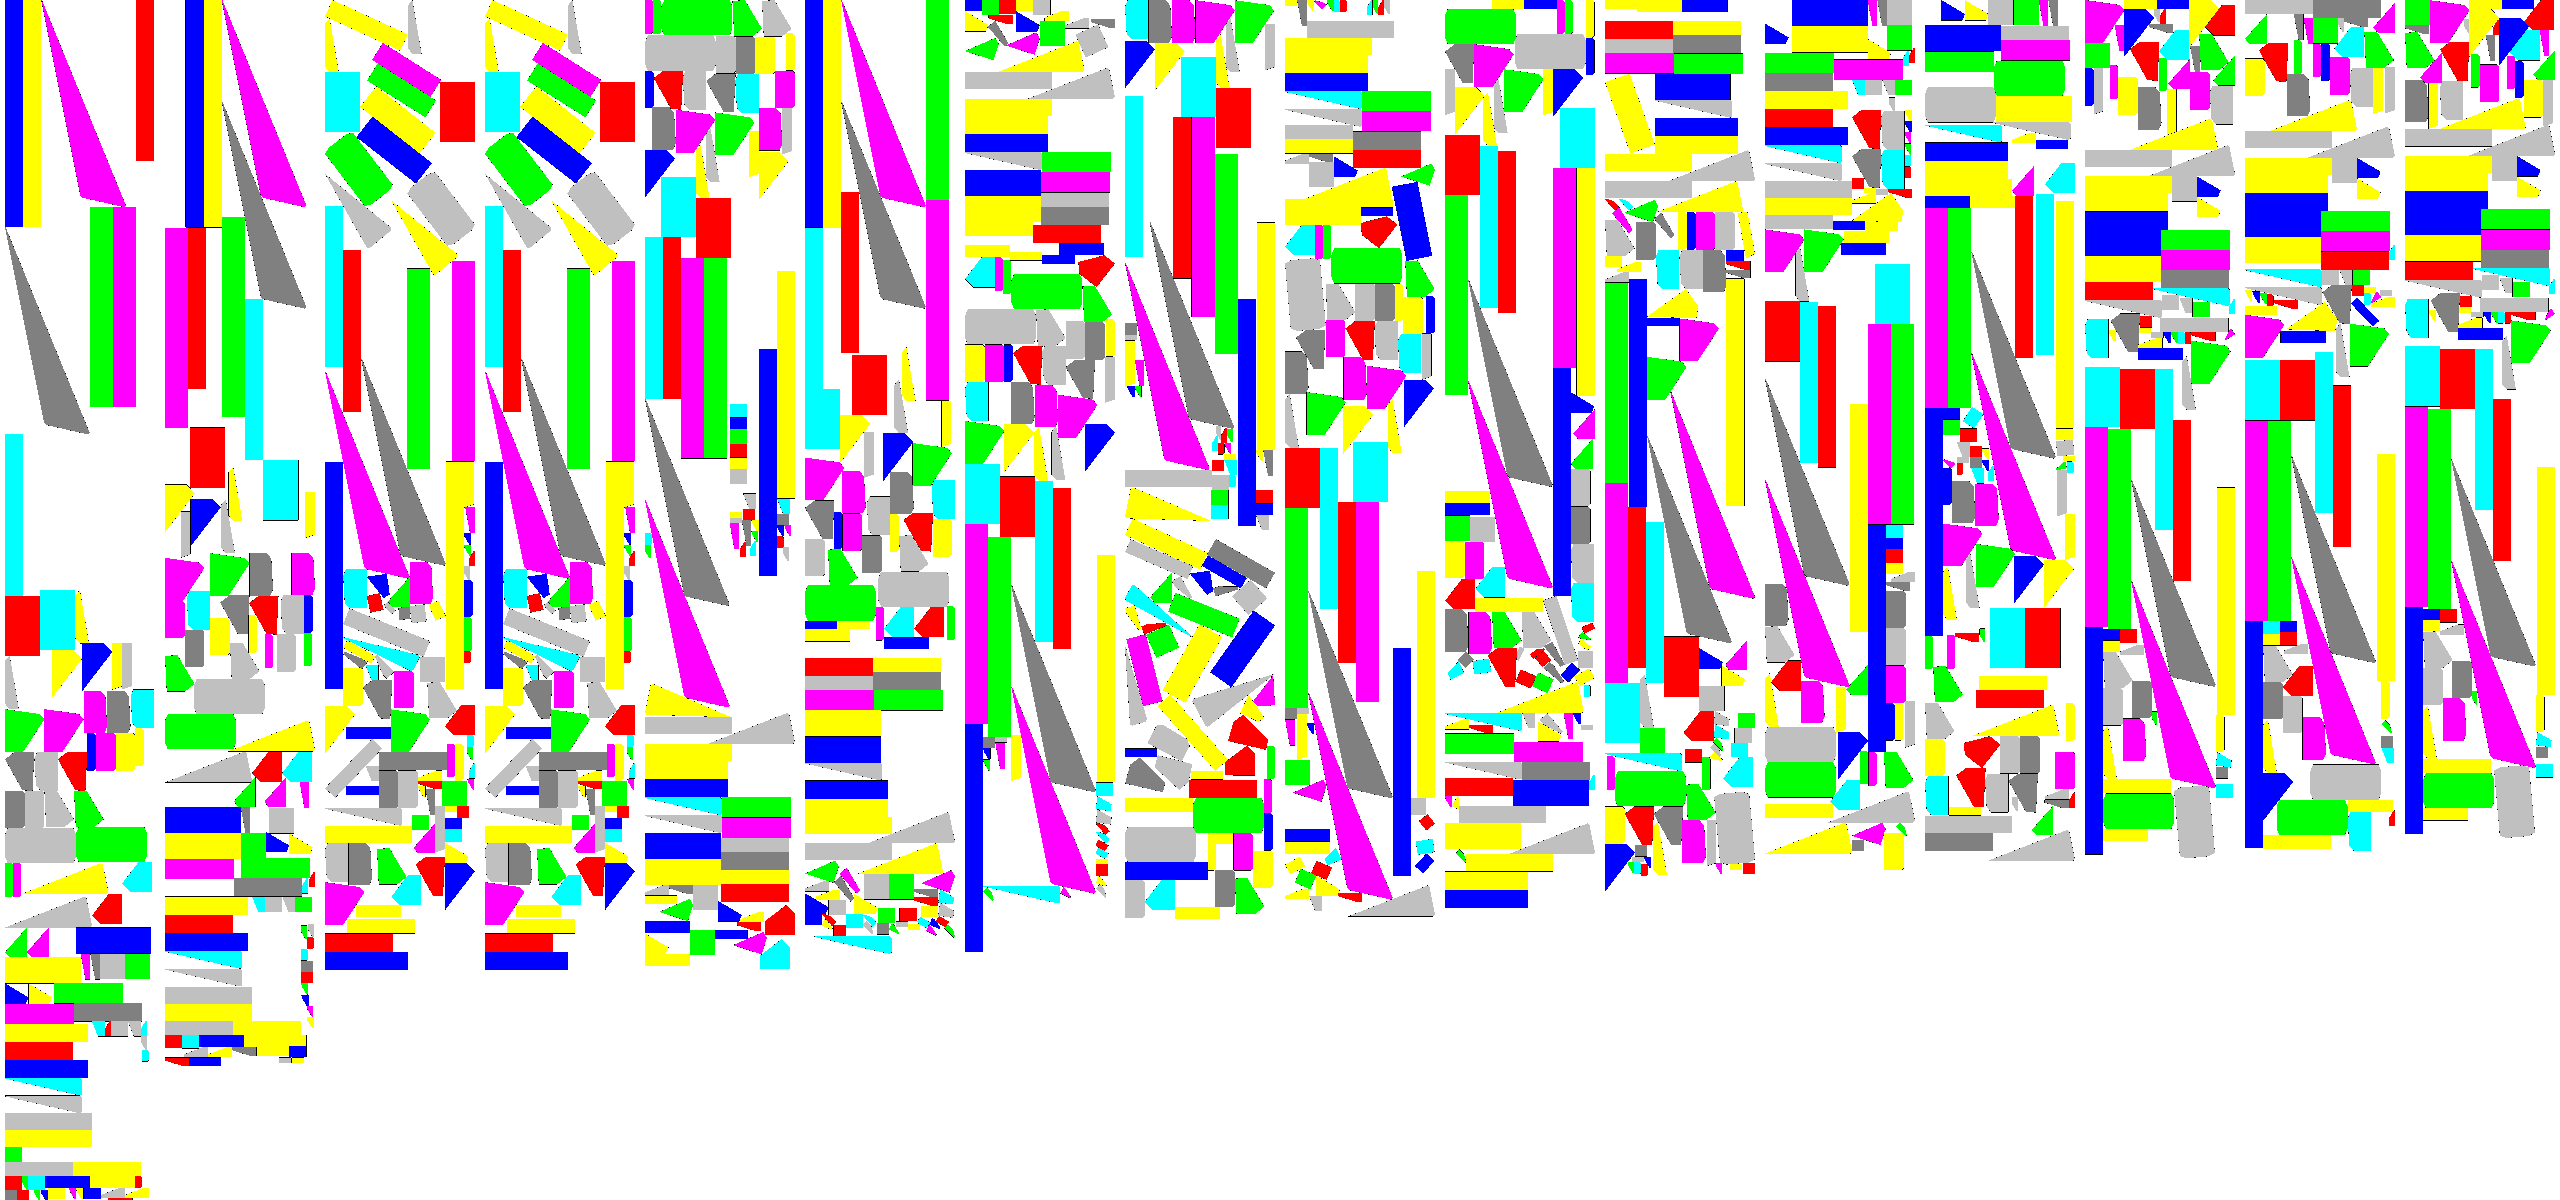
\includegraphics[width=12.62cm,height=7.88cm]{fig01.png}
	\caption{Experiment 1 - final packing solution.}
	\label{fig:Graph}
\end{figure}
%
\begin{figure}
	\centering
	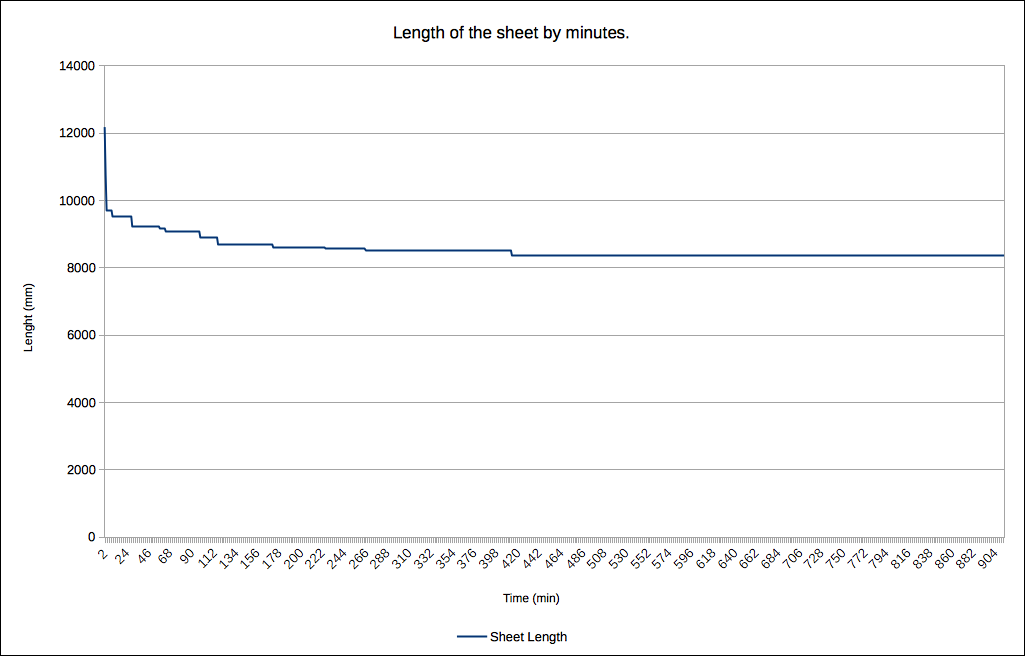
\includegraphics[width=12.62cm,height=7.88cm]{fig02.png}
	\caption{Experiment 2 - final packing solution.}
	\label{fig:Graph}
\end{figure}
%
\begin{figure}
	\centering
	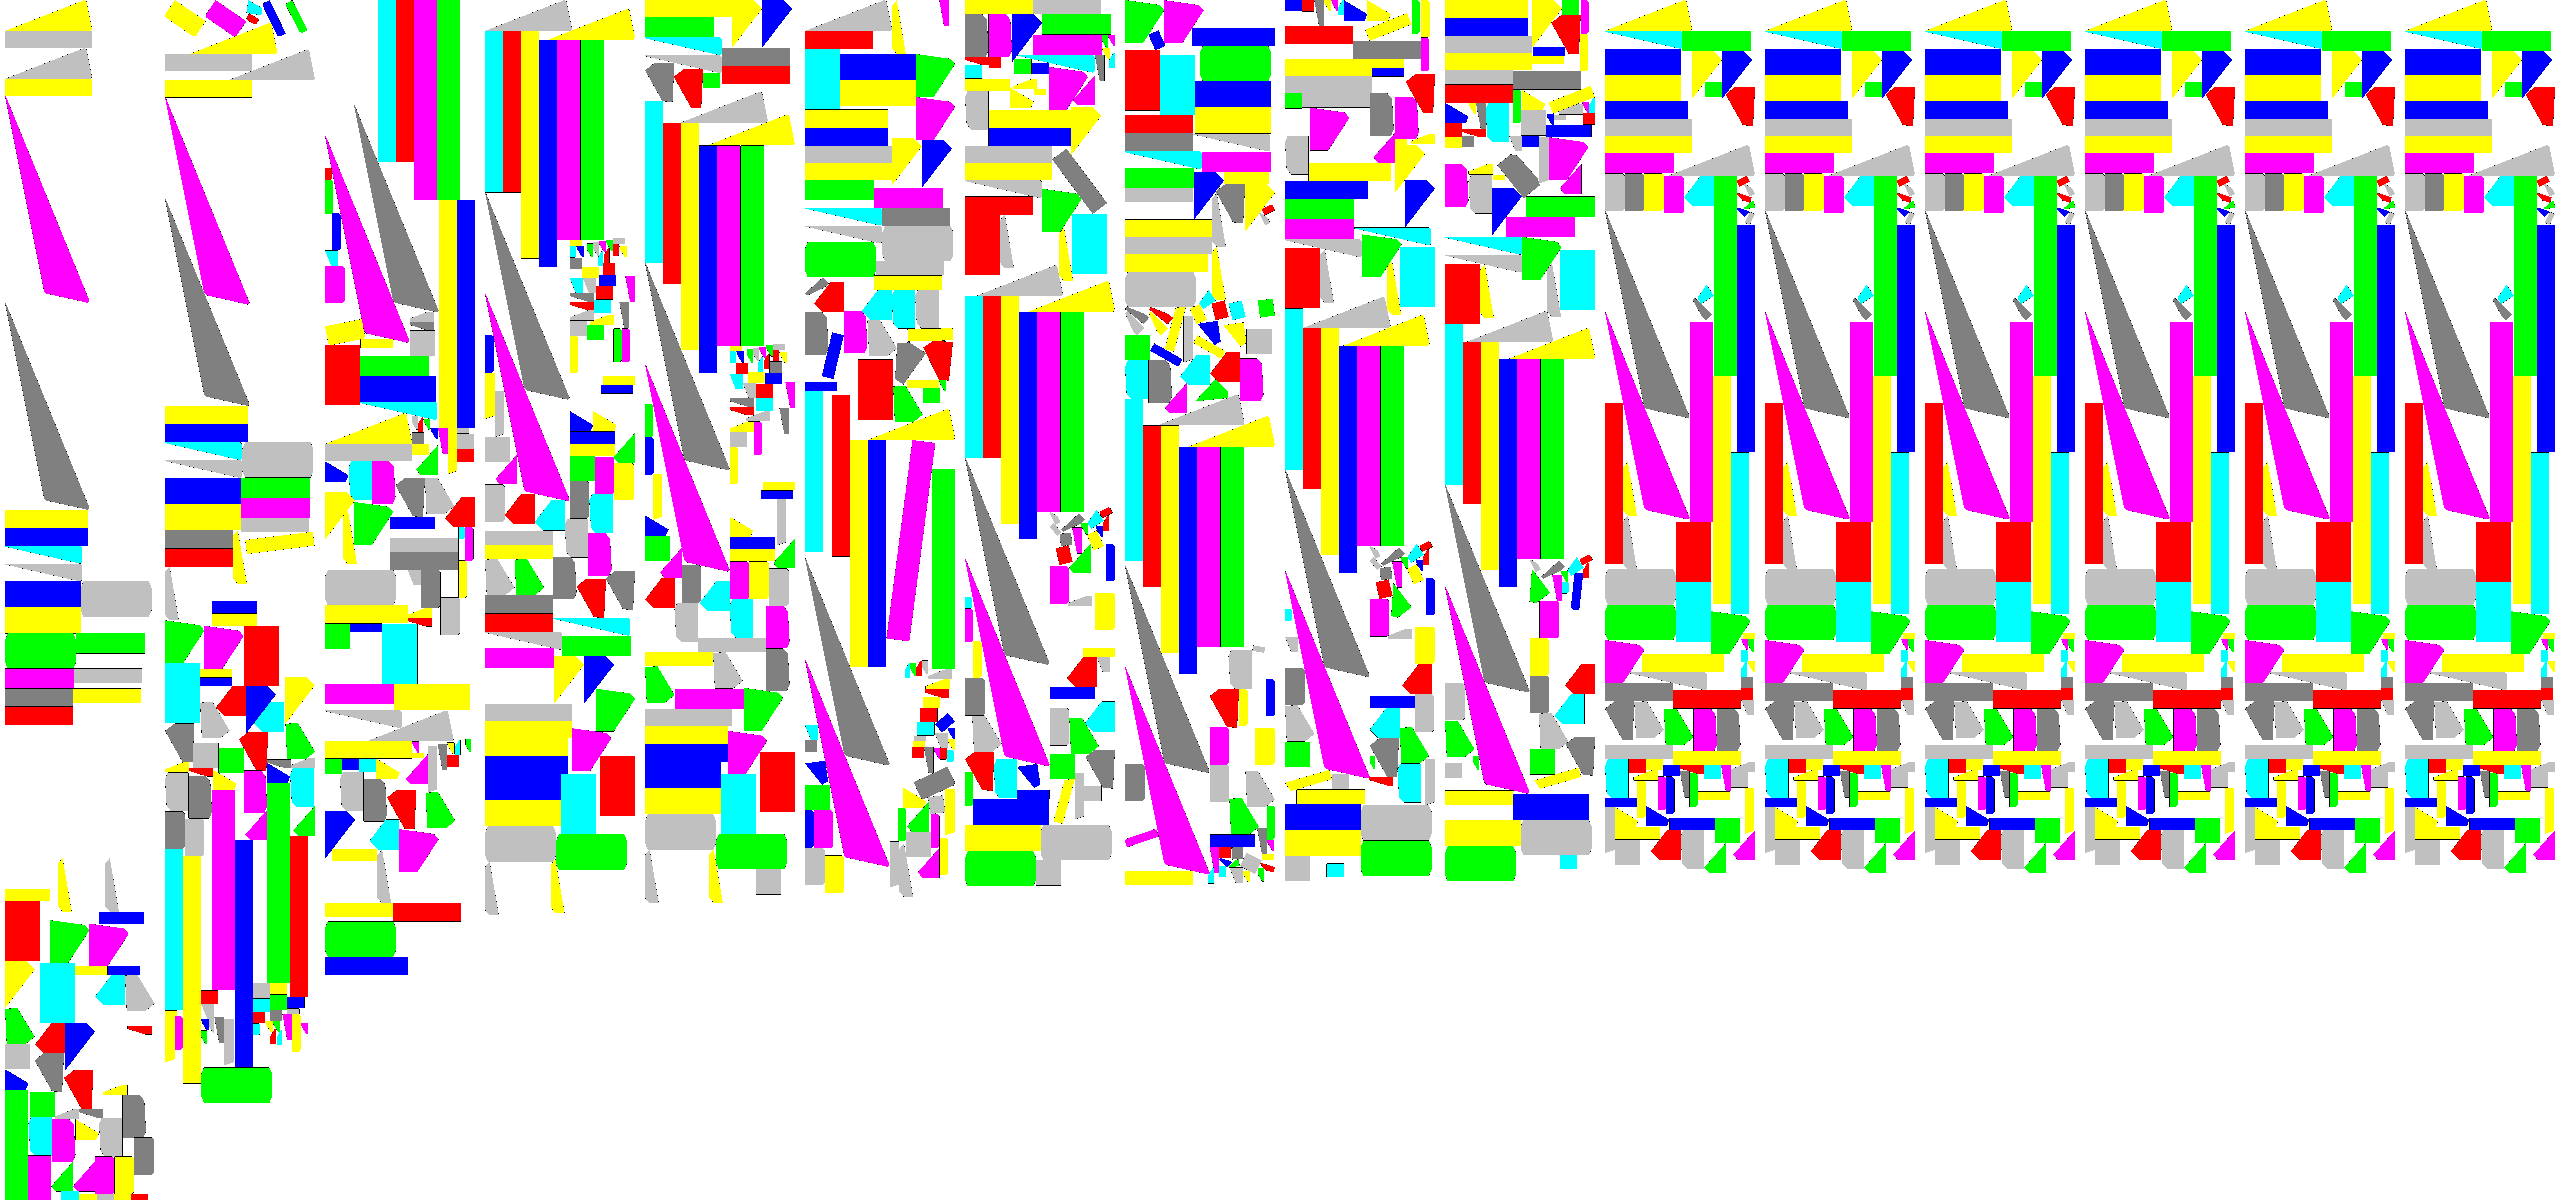
\includegraphics[width=12.62cm,height=7.88cm]{fig03.png}
	\caption{Experiment 3 - final packing solution.}
	\label{fig:Graph}
\end{figure}
\FloatBarrier

The convergence of the experiments is similar as it is shown on Fig. 4. Convergence is stairs like because GA is working on a discrete basis and elitism rule was applied.

\begin{figure}
	\centering
	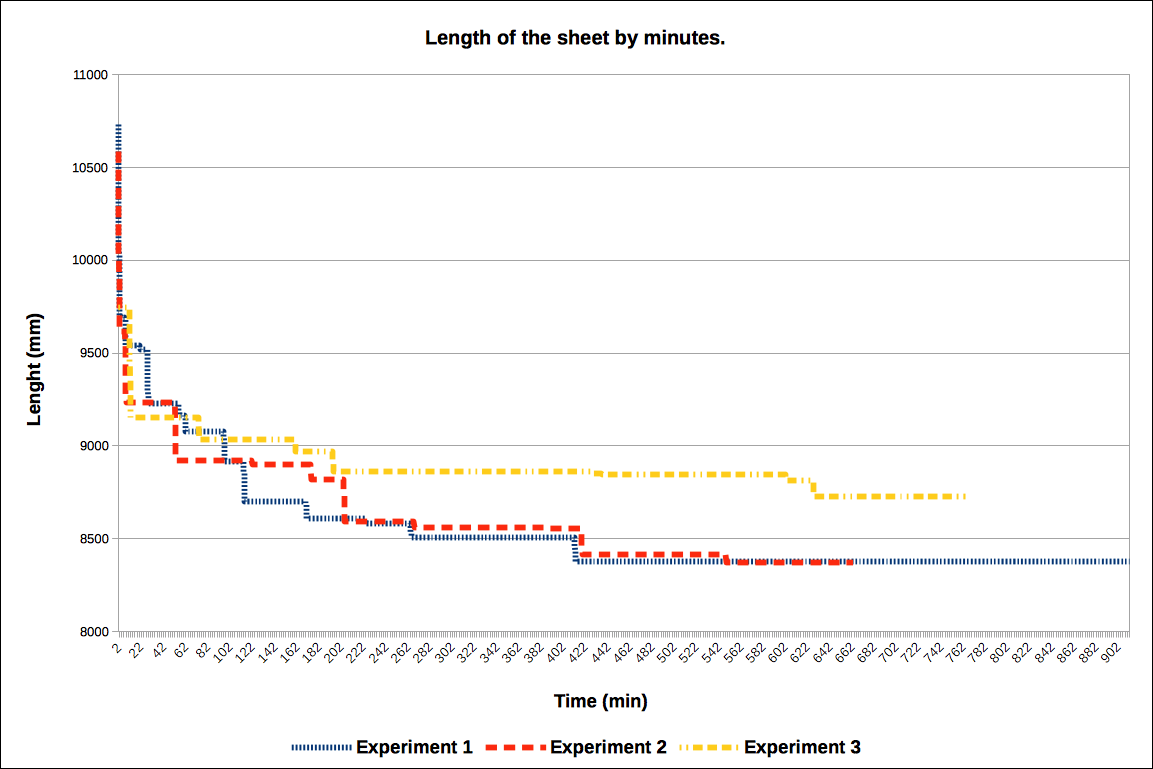
\includegraphics[width=12.62cm,height=7.88cm]{fig05.png}
	\caption{Optimization convergence comparison. On the Y-axis the length of the used steel sheet is presented. On the X-axis optimization time is presented (in minutes) on an average performing laptop.}
	\label{fig:Graph}
\end{figure}
\FloatBarrier
%
It is obvious that the two biggest triangles are problematic in the optimal packing and GA is not very capable to deal with this local optima problem.
%
\section{Conclusions}
%
Usage of GAs for PIS is a promising approach, but solutions are suboptimal and relatively far away from the global optimum. In real industrial application GA may be combined with interactive human assistance in order to achive faster and better solutions. 
%
\section*{Acknowledgements}
%
%
This work was supported by private funding of Velbazhd Software LLC.
%
% ---- Bibliography ----
%
\begin{thebibliography}{}
%
\bibitem {evti:fid}
Evtimov, G., Fidanova, S.:
Ant Colony optimization algorithm for 1D Cutting Stock Problem.
Proceedings of 11th Annual Meeting of the Bulgarian Section of SIAM, FASTUMPRINT, Sofia, Bulgaria, 24--25 (2016)
%
\bibitem {evti}
Evtimov, G.:
Project 2: Optimal cutting problem.
STOBET Ltd., 120th European Study Group with Industry, Sofia, Bulgaria  (2016)
%
\bibitem {bal:evti}
Balabanov, T., Evtimov, G., Koleva, D.:
ESGI 120 - Problem 2 - Genetic Algorithm Solver.
https://github.com/VelbazhdSoftwareLLC/ESGI120Problem2GeneticAlgorithmSolver Sofia, Bulgaria  (2016)
%
\bibitem {avdz:bal}
Avdzhieva, A., Balabanov, T., Evtimov, G., Kirova, D., Kostadinov, H., Tsachev, Ts., Zhelezova, S., Zlateva N.:
Optimal Cutting Problem.
Problems \& final reporst of 113-th European Study Group with Industry, FASTUMPRINT, Sofia, Bulgaria, 49--61 (2015)
%
\bibitem {mart:mon}
Martelloa, S., Monacib, M.:
Models and algorithms for packing rectangles into the smallest square.
Computers \& Operations Research, vol. 63, 161--171 (2015)
%
\bibitem {bal:1}
Balabanov, T.:
Distributed evolutional model for music composition by human-computer interaction.
Proceedings of International Scientific Conference UniTech15, University publishing house V. Aprilov, Gabrovo, Bulgaria, vol. 2, 389--392 (2015)
%
\bibitem {bal:2}
Balabanov, T.:
Avoiding Local Optimums in Distributed Population based Heuristic Algorithms (in Bulgarian).
Proceedings of XXIII International Symposium Management of energy, industrial and environmental systems, John Atanasoff Union of Automation and Informatics, Sofia, Bulgaria, 83--86 (2015)
%
\bibitem {bal:3}
Balabanov, T.:
Heuristic Forecasting Approaches in Distributed Environment (in Bulgarian).
Proceedings of Anniversary Scientific Conference 40 Years Department of Industrial Automation, UCTM, Sofia, Bulgaria, 163--166 (2011)
%
\bibitem {tere:mig}
Teresa Costa, M.,  Miguel Gomes, A., Oliveira, J.:
Heuristic approaches to large-scale periodic packing of irregular shapes on a rectangular sheet.
European Journal of Operational Research, vol. 192, 29--40 (2009)
%
\bibitem {dows:dows}
Dowsland, K., Dowsland, W.:
Packing problems.
European Journal of Operational Research, vol. 56, 2--14 (1992)
%
\end{thebibliography}
\end{document}
